\documentclass{tufte-book}

\title{Mastering KiCad Version 5.0\thanks{Thanks to all the KiCad developers for their tireless efforts.}}
\author[Seth Hillbrand]{Seth~Hillbrand}
\publisher{}


\usepackage{fontenc}
\setmainfont[Renderer=Basic, Scale = 1.0, SmallCapsFont={Cormorant SC}]{Cormorant}
\setsansfont[Renderer=Basic, Scale=0.90]{Lato Regular}
\setmonofont[Renderer=Basic, Scale=0.80]{Cousine}

\usepackage{microtype}
\usepackage{booktabs}
\usepackage{graphicx}
\setkeys{Gin}{width=\linewidth,totalheight=\textheight,keepaspectratio}
\graphicspath{{graphics/}}

\usepackage{geometry}
\geometry{  paperwidth = 7in,
			paperheight = 10in,
			left = 1in,
			top = 1in,
			headsep=2\baselineskip,
			textwidth=24pc,
			marginparsep=1pc,
			marginparwidth=10pc,
			textheight=44\baselineskip,
			headheight=\baselineskip
			 }

\usepackage{fancyvrb}
\fvset{fontsize=\normalsize}

% Hanging paren
\newcommand{\hangp}[1]{\makebox[0pt][r]{(}#1\makebox[0pt][l]{)}}

% Hanging asterix
\newcommand{\hangstar}{\makebox[0pt][l]{*}}

\usepackage{xspace}


% Prints the month name (e.g., January) and the year (e.g., 2008)
\newcommand{\monthyear}{%
  \ifcase\month\or January\or February\or March\or April\or May\or June\or
  July\or August\or September\or October\or November\or
  December\fi\space\number\year
}

\newcommand{\blankpage}{\newpage\hbox{}\thispagestyle{empty}\newpage}

% Macros for typesetting the documentation
\newcommand{\hlred}[1]{\textcolor{Maroon}{#1}}% prints in red
\newcommand{\hangleft}[1]{\makebox[0pt][r]{#1}}
\newcommand{\hairsp}{\hspace{1pt}}% hair space
\newcommand{\hquad}{\hskip0.5em\relax}% half quad space
\newcommand{\TODO}{\textcolor{red}{\bf TODO!}\xspace}
\newcommand{\na}{\quad--}% used in tables for N/A cells

\newcommand{\tuftebs}{\symbol{'134}}% a backslash in tt type in OT1/T1
\newcommand{\doccmdnoindex}[2][]{\texttt{\tuftebs#2}}% command name -- adds backslash automatically (and doesn't add cmd to the index)
\newcommand{\doccmddef}[2][]{%
  \hlred{\texttt{\tuftebs#2}}\label{cmd:#2}%
  \ifthenelse{\isempty{#1}}%
    {% add the command to the index
      \index{#2 command@\protect\hangleft{\texttt{\tuftebs}}\texttt{#2}}% command name
    }%
    {% add the command and package to the index
      \index{#2 command@\protect\hangleft{\texttt{\tuftebs}}\texttt{#2} (\texttt{#1} package)}% command name
      \index{#1 package@\texttt{#1} package}\index{packages!#1@\texttt{#1}}% package name
    }%
}% command name -- adds backslash automatically
\newcommand{\doccmd}[2][]{%
  \texttt{\tuftebs#2}%
  \ifthenelse{\isempty{#1}}%
    {% add the command to the index
      \index{#2 command@\protect\hangleft{\texttt{\tuftebs}}\texttt{#2}}% command name
    }%
    {% add the command and package to the index
      \index{#2 command@\protect\hangleft{\texttt{\tuftebs}}\texttt{#2} (\texttt{#1} package)}% command name
      \index{#1 package@\texttt{#1} package}\index{packages!#1@\texttt{#1}}% package name
    }%
}% command name -- adds backslash automatically
\newcommand{\docopt}[1]{\ensuremath{\langle}\textrm{\textit{#1}}\ensuremath{\rangle}}% optional command argument
\newcommand{\docarg}[1]{\textrm{\textit{#1}}}% (required) command argument
\newenvironment{docspec}{\begin{quotation}\ttfamily\parskip0pt\parindent0pt\ignorespaces}{\end{quotation}}% command specification environment
\newcommand{\docenv}[1]{\texttt{#1}\index{#1 environment@\texttt{#1} environment}\index{environments!#1@\texttt{#1}}}% environment name
\newcommand{\docenvdef}[1]{\hlred{\texttt{#1}}\label{env:#1}\index{#1 environment@\texttt{#1} environment}\index{environments!#1@\texttt{#1}}}% environment name
\newcommand{\docpkg}[1]{\texttt{#1}\index{#1 package@\texttt{#1} package}\index{packages!#1@\texttt{#1}}}% package name
\newcommand{\doccls}[1]{\texttt{#1}}% document class name
\newcommand{\docclsopt}[1]{\texttt{#1}\index{#1 class option@\texttt{#1} class option}\index{class options!#1@\texttt{#1}}}% document class option name
\newcommand{\docclsoptdef}[1]{\hlred{\texttt{#1}}\label{clsopt:#1}\index{#1 class option@\texttt{#1} class option}\index{class options!#1@\texttt{#1}}}% document class option name defined
\newcommand{\docmsg}[2]{\bigskip\begin{fullwidth}\noindent\ttfamily#1\end{fullwidth}\medskip\par\noindent#2}
\newcommand{\docfilehook}[2]{\texttt{#1}\index{file hooks!#2}\index{#1@\texttt{#1}}}
\newcommand{\doccounter}[1]{\texttt{#1}\index{#1 counter@\texttt{#1} counter}}

% Generates the index
\usepackage{makeidx}


\makeindex

\begin{document}
\frontmatter
\blankpage
{
  \let\allcaps=\relax
  \maketitle
}

\newpage
\begin{fullwidth}
~\vfill
\thispagestyle{empty}
\setlength{\parindent}{0pt}
\setlength{\parskip}{\baselineskip}
Copyright \copyright\ \the\year\ \thanklessauthor

\par\smallcaps{Published by \thanklesspublisher}

\par\smallcaps{https://mastering-kicad.github.io/v5}

\par This work is licensed under the Creative Commons Attribution 4.0 International License (the ``License''). 
To view a copy of this license, visit \url{http://creativecommons.org/licenses/by/4.0/} or send a letter to Creative Commons, PO Box 1866, Mountain View, CA 94042, USA. 

\par Code samples included in this book are licensed under the terms of the GNU General Public License as published by the Free Software Foundation, either version 3 of the License, or (at your option) any later version. 
To view a copy of this license, visit \url{https://www.gnu.org/licenses/gpl-3.0.html}.\index{license}

\par\textit{First printing, \monthyear}
\end{fullwidth}

\tableofcontents

\listoffigures

\listoftables

\cleardoublepage
~\vfill
\begin{doublespace}
\noindent\fontsize{18}{22}\selectfont\itshape
\nohyphenation
Dedicated to people \TODO Insert ded.
\end{doublespace}
\vfill
\vfill


\cleardoublepage
\chapter*{Introduction}

\newthought{A project like KiCad} does not have a single or even primary person who is responsible for the plurality of the work.
Instead, there are many, many individuals, spread across the globe who come together over mailing lists and bug trackers to create something as a whole.
People will often drift into and out of such endeavors as their time and inclination permits.
But they leave a last, indelible and -- hopefully -- positive impact on the codebase, user experience, libraries, documentation and artwork that make up the amazing ecosystem of KiCad.

That said, a few individuals' contributions help to ensure that the ecosystem exists in the first place, that contributors are encouraged and that activity is focused where it will do the most good.
KiCad is fortunate to have (and have had) the contributions of Jean-Pierre Charras, whose work has been the foundation of KiCad and whose continued contribution to its development is an example of selfless dedication.
In addition, Dick Hollenbeck and his employer SoftPLC contributed a substantial fraction of the KiCad internals and structure.
Wayne Stambaugh who, in his role as project leader, has guided the KiCad team since 2014 and provided a much-needed steadying hand as the project developed into what it is today.
In addition to these three, there are many, many more dedicated, collaborative developers working to make KiCad stronger.

Part of making KiCad stronger is introducing it to a wider audience and, hopefully, reducing some of the headaches that accompany learning a new piece of software.
That is what I hope this book will provide.
This book is meant to supplement rather than supplant the official KiCad documentation\sidenote{\url{http://kicad-pcb.org/help/documentation/}}.
While intended aimed primarily at a University audience learning KiCad and PCB design simultaneously, I hope that it also provides a helpful reference for regular KiCad users looking to improve their usage patterns.

\mainmatter

%!TEX root = ../main.tex

\chapter{Introduction to KiCad}
\label{ch:intro-kicad}

`

\section{Circuit Design}


\section{Prototyping}

\section{Printed Circuit Boards}

\section{Installing KiCad}
\subsection{Linux}
\subsection{MacOS}
\subsection{Windows}

\section{Installing Libraries and Models}

\section{First Run}
\subsection{Setup Paths}
\subsection{Setup Symbol Library Table}
\subsection{Setup Footprint Library Table}

\section{Upgrading from Version 4}

\section{Opening Example Projects}

\section{Summary}
%%!TEX root = ../main.tex

\chapter{KiCad Design Workflow}
\section{Project Initialization}
\section{Component Selection}
\section{Schematic Layout}
\section{Electrical Rules Check}
\section{Footprint Association}
\section{Circuit Board Layout}
\section{Design Rules Check}
\section{Generating Design Files}
\subsection{Gerber Files}
\subsection{IPC Files}
\subsection{XY Placement Files}
%%!TEX root = ../main.tex

\chapter{KiCad Project Structure}
\label{ch:project-structure}

\section{Using Git}
\subsection{Version Control Basics}
\subsection{Local vs. Remote}
\subsection{Shallow Copies}
\subsection{Personal Libraries}

\section{Building Robust Projects}

\section{Template Design}

\section{KiCad Component Libraries Explained}
\subsection{Symbol Library Management}
\subsection{Footprint Library Management}

\section{Project Files and Sub-files}
%%!TEX root = ../main.tex

\chapter{Component Symbol Design and Library Management}

Components in KiCad represent the electrical state of a single element in the schematic.
They also map the pin numbers of the element to a descriptive pin name.

In the schematic, we wire connections to pins based on their names and idiomatic positions.
The netlist is then generated using the pin number to map the schematic to the physical connections on the circuit board.

KiCad has a group of dedicated librarians who design, organize and curate a library of more than 10,000 symbols that are free to download at \url{https://kicad.github.io/symbols/}.  
Each symbol represents a distinct part.

\section{Libraries, Parts and Aliases}

In general, there are two types of symbols in the KiCad libraries: Atomic and Generic.
A Generic part is one for which there are many possible footprints and variations.
Examples of Generic parts are \textit{Resistors}, \textit{Capacitors}, \textit{BJTs} and similar parts.

Generic parts will typically not have footprints, footprint filters, manufacturer part numbers or similar identifying characteristics as there are many variations for each.

Atomic parts, on the other hand represent a specific manufacturer part.
These will typically have their associated datasheet, mpn and footprint assigned in the library.

Many components have alternate versions for small variations such as temperature or voltage compliance.
Where the pin numbers do not change between variations, we typically utilize \textit{aliases}.
An alias of a part is a component with the same pin number to pin name mapping but different part name and potentially different footprint, documentation and part description.

\section{KLC Design Guidelines}

The Kicad Library Convention (KLC) provides design guidelines for the creation of KiCad-like parts.
While nothing in the underlying KiCad code prevents you from breaking the convention, the KLC provides stylistic guidelines that will help your parts to work well with the existing libraries.
They are also required if and when you decide to submit your library parts for inclusion in the KiCad distribution.



\section{Graphic Items}

\section{Pins}
\subsection{Pin Names}
\subsection{Pin Numbers}
\subsection{Pin Types}
\subsection{Pin Stacking}
\subsection{Pin Table}

\section{Multi-unit Parts}
\subsection{De Morgan Parts}
\subsection{Heterogenous Parts}
\subsection{Homogeneous Styles}

\section{Field Properties}
\subsection{Footprints}
\subsection{Documentation}
\subsection{Keywords}

\section{Tips and Tricks for Common Mistakes}

\section{Symbol Design Examples}
\subsection{Example 1: Basic Symbol}
\subsection{Example 2: Heterogenous, Multi-unit Symbol}
%%!TEX root = ../main.tex

\chapter{Schematic Editor}

The first step in every project is schematic capture.
If this term is unfamiliar, we are referring to the process of laying out the components and connections between them in logical, well-defined fashion.
You may have only the barest idea of the circuit aspects or you may have the major aspects already sketched on paper;
whatever your situation, transferring the schematic into KiCad begins with the Schematic Editor.

Before we dive into the simplistic aspects of the schematic editor, it will pay us dividends later to properly understand how the schematic editor views more complex schematics.
This will allow you to structure the schematic in your mind more closely to how Schematic Editor expects.

\section{Hierarchical Schematics Explained}

The basic, underlying paradigm of the Schematic Editor is the idea of \textit{hierarchical schematics}.
If the overall schematic represents the full circuit that will exist on the circuit board at the end of production, then the hierarchy provides a logical grouping of similar component sets.
This allows you to reuse common subsets throughout your design.
The hierarchy also explicitly structures your schematics as a top-down tree.
\begin{figure}
	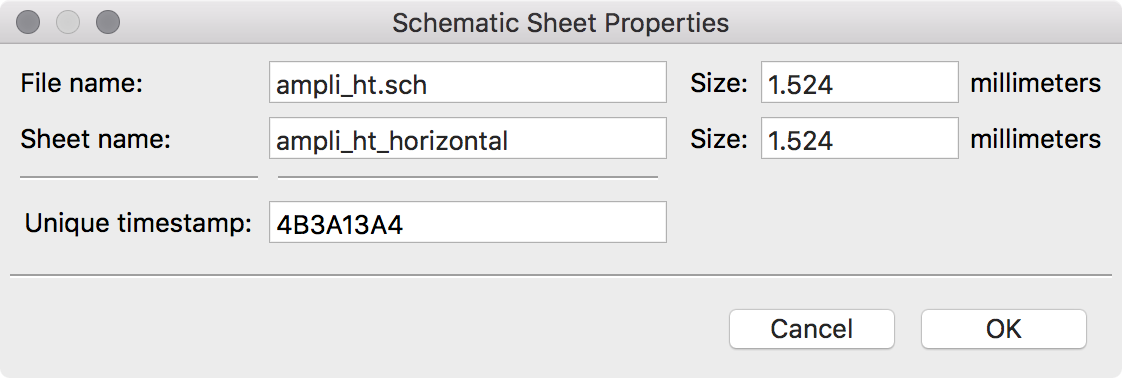
\includegraphics{chapter5/subsheet.png}
	\caption[Sub-Sheets]{The subsheet dialog specifies the file name, sheet name and a unique timestamp.}
\end{figure}

At the root of the tree, is the first schematic sheet you open, usually with the same name as your project and the extension `\textbf{.sch}'.
Off of this root, you can create \textit{sub-sheets} that are placed in the root sheet.
The sub-sheet has both a ``File name'' and a ``Sheet name''.
The File name is the name of the sub-sheet on the underlying filesystem.
This is the name you will see if you open your project folder outside of KiCad.
The Sheet name is the internal reference of the specific \textit{instance} of the sub-sheet in KiCad.

One of the primary benefits of this setup is the ability to organize the relationship between subsheets.
It can also allow you to create and re-use common elements between projects.
This will be useful when we begin discussing design reuse in section \ref{sec:reuse}.


\section{Understanding the Schematic Editor}
\begin{figure*}
    \begin{tikzpicture}
    \node [anchor=west] (note) at (-1,3) {\Large Note};
    \node [anchor=west] (water) at (-1,1) {\Large Water};
    \begin{scope}[xshift=0.5cm]
        \node[anchor=south west,inner sep=0] (image) at (0,0) {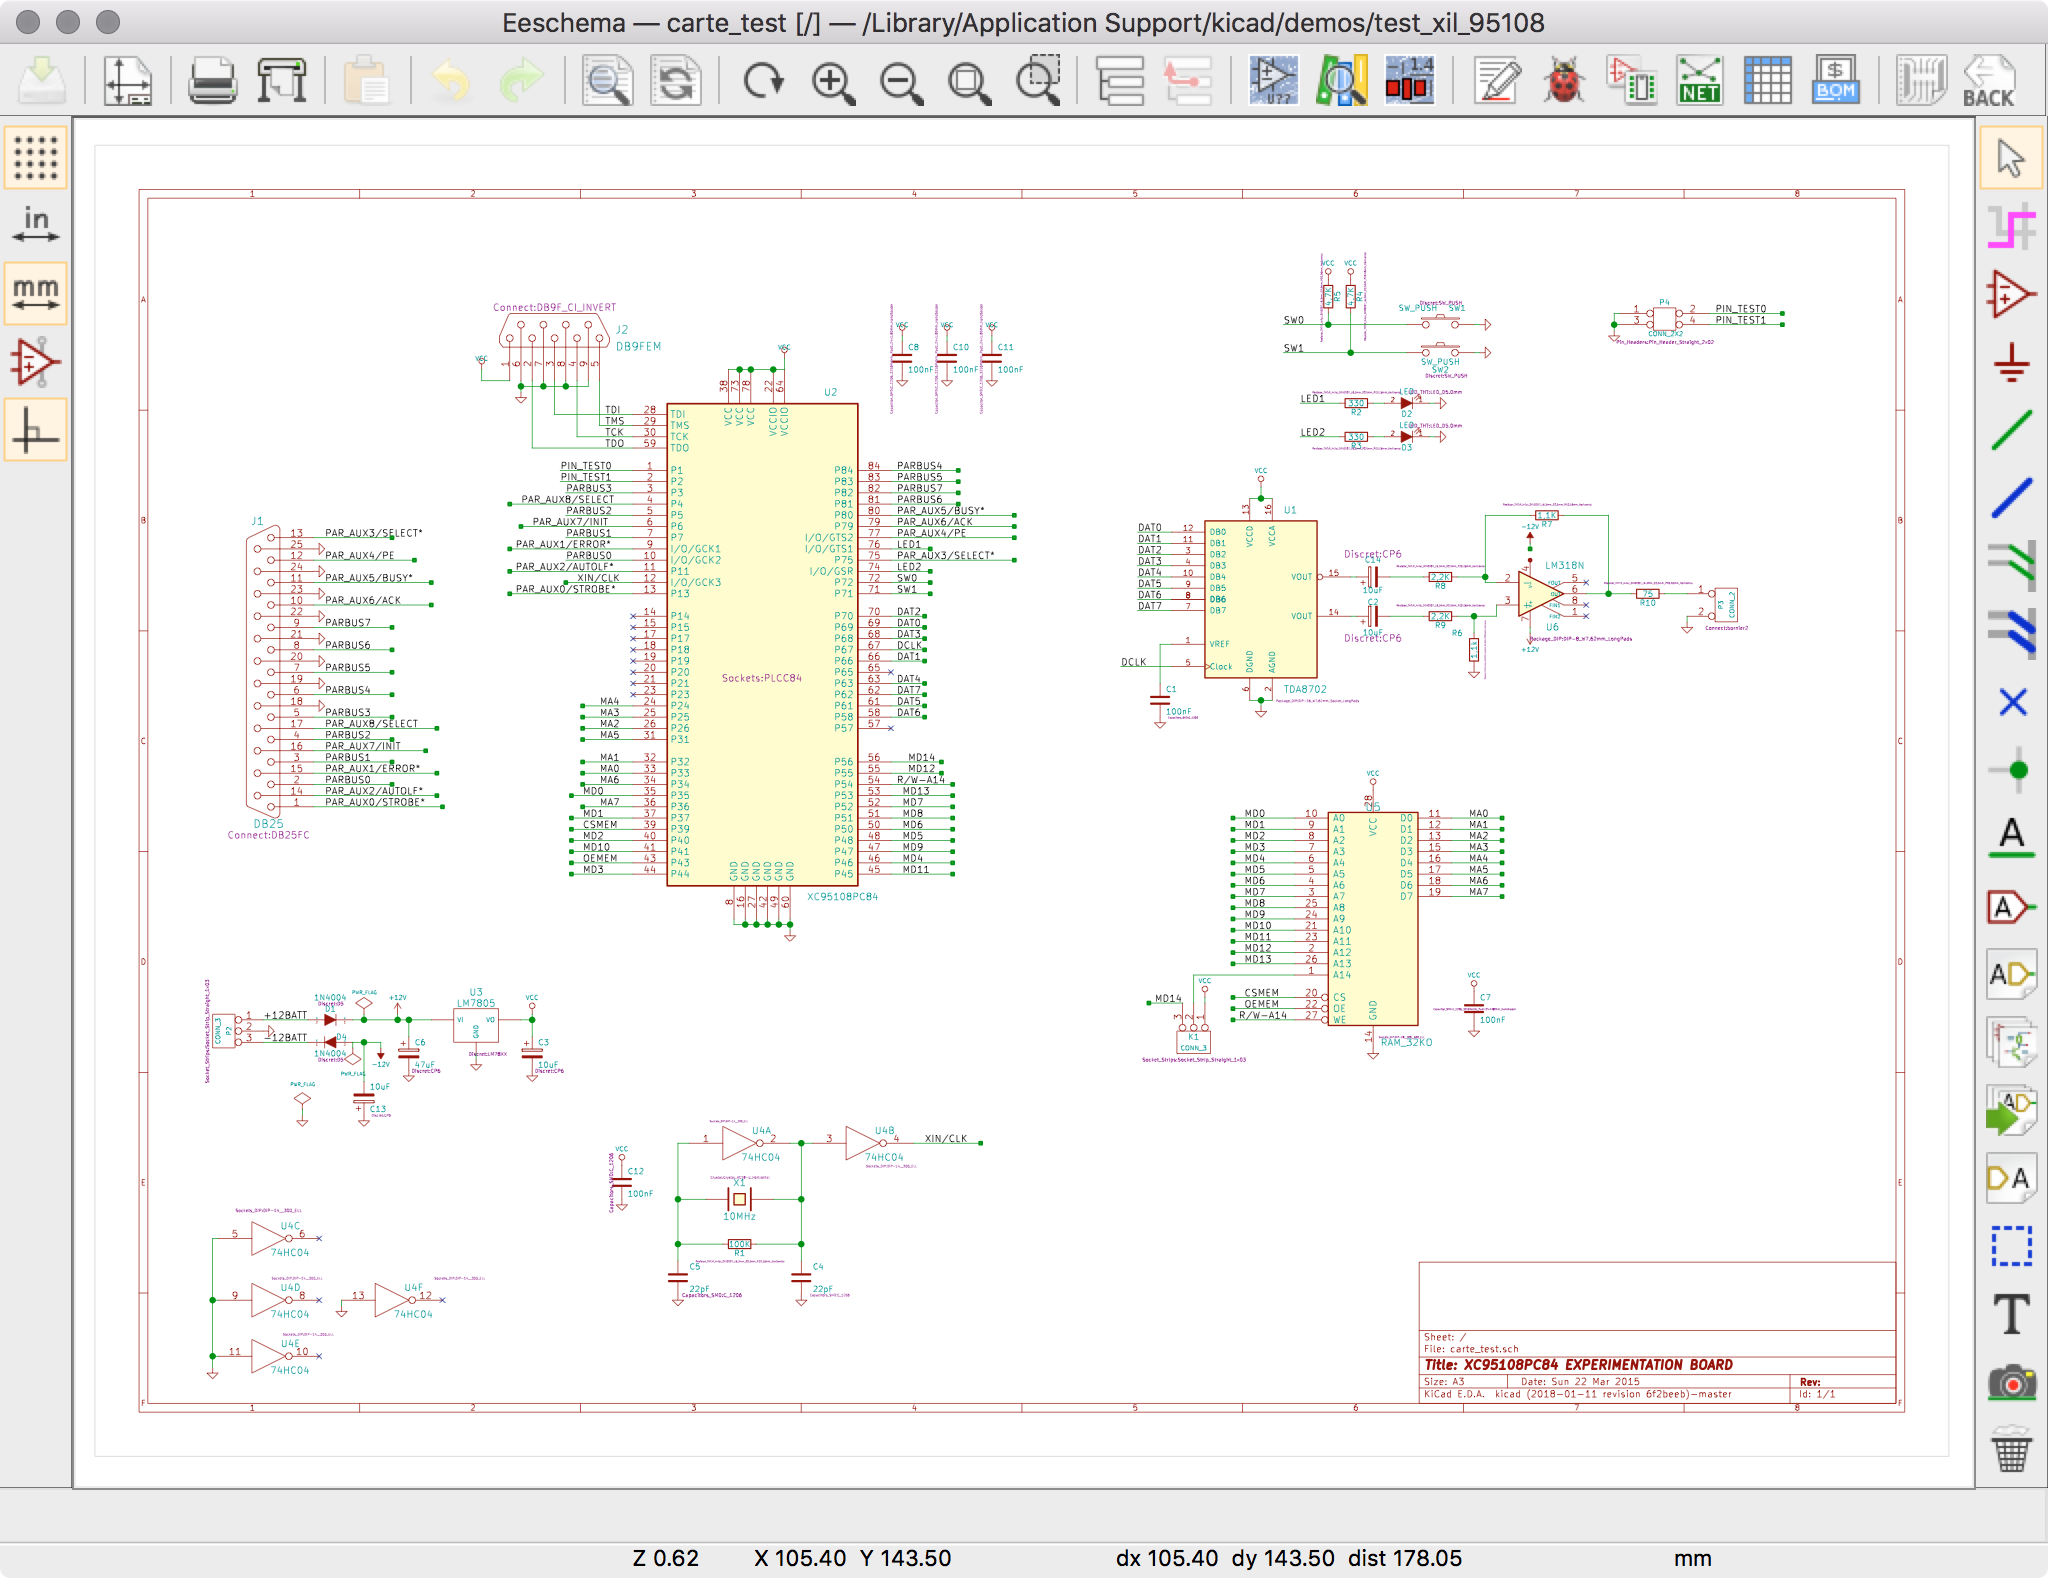
\includegraphics[width=4.5in]{chapter5/eeschema-main.png}};
        \begin{scope}[x={(image.south east)},y={(image.north west)}]
            \draw[help lines,xstep=.05,ystep=.05] (0,0) grid (1,1);
            \draw[red,thick,rounded corners] (0.38,0.90) rectangle (1.55,1.0);
            \draw [-latex, ultra thick, red] (note) to[out=0, in=-120] (0.48,0.80);
            \draw [-stealth, line width=5pt, cyan] (water) -- ++(0.4,0.0);
        \end{scope}
    \end{scope}
    \end{tikzpicture}
	
	\caption[Eeschema]{The Eeschema main window}
\end{figure*}
\subsection{Relationship to Symbol Libraries}
\subsection{Project Settings}

\section{Adding Parts}

\section{Connections}
\subsection{Wires}
\subsection{Busses}
\subsection{Labels}
\subsection{Junctions}
\subsection{No Connects}
\subsection{Hierarchical Pins}

\section{Electrical Rules Check}

\section{Graphical Elements}

\section{Templates}

\section{Schematic Editor Examples}
\subsection{Example 1: Single Page Schematic}
\subsection{Example 2: Hierarchical Schematic}
%%!TEX root = ../main.tex

\chapter{Footprint Design with KiCad}

Through a dedicated team of volunteer librarians, KiCad provides an incredible assortment of footprints.
Sometimes, however, you will find that you need a footprint that does not yet exist in the provided libraries.
Or, worse, the provided footprint isn't exactly what you need to match your build requirements.
For these cases, KiCad provides an extremely powerful, if not terribly intuitive, footprint design program.

\section{Footprint Types}
In this chapter, we will walk you through the basics of footprint design for surface mount components (SMDs), through-hole components (THTs) and virtual components\sidenote{Virtual components are elements that exist only on the board itself.  
Examples include antennas that are printed into the copper cladding and connector fingers on the board edge}.

\subsection{Through hole}

Through hole components are ubiquitous, easy to work with, easy to replace and easy to debug.  
For these reasons, through hole components are often the first element designers reach for when building a simple circuit.  
One downside, however is that through-hole components are physically large.  
They need to leave enough room to have a hole that goes through the circuit board, the annular ring around the hole and then clearance to the next hole.
This limits their usability in small spaces and at high frequencies.

A second downside is that, because the connection pin extends through the full circuit board, it places on a barrier for any traces on layers under the pin.  
With may through hole components placed closely together, the barrier can be substantial and set up `walls' that impede ground planes and signal traces.

\subsection{SMD}

Surface mount components overcome many of the shortcomings of THT components by making the electrical contact points flat pins or plates that are soldered to exposed pads on the circuit board.
SMDs are also ubiquitous but are harder to work with, harder to replace and harder to debug.
All of these drawbacks are the result of SMDs addressing the major shortcoming of the THT components: their size.
SMD components are almost arbitarily small and can fit a dizzying number of connections inside of a very small package.


\subsection{Virtual}

Virtual components can be extremely useful when used properly.
They rely on using the physical properties of the cladding to acheive a specific result in your circuit.
Whether this is designing a 0.1pF capacitor, creating an on-board antenna or placing edge fingers to connect your circuit board

\section{Layers}

\section{Pins and Pads}
\subsection{Pad Shapes}
\subsection{Custom Shapes}
\subsection{Masks}
\subsection{Special Pins}

\section{Clearance Settings}

\section{Thermal Relief}

\section{3d Settings}

\section{Creating Footprints using Generators}

\section{Footprint Design Examples}
\subsection{Example 1: QFN with Exposed Pad}
\subsection{Example 2: High-Density, Through-hole Connector}
\subsection{Example 2: Board-Edge Connector}
%%!TEX root = ../main.tex

\chapter{Printed Circuit Board Layout}
\label{ch:pcbnew}

\section{Basic Board Settings}

\section{Board Layers}
\subsection{Layer Pairs}
\subsection{Special Layers}
\subsection{User Layers}
\subsection{Customizing your Layers}

\section{Adding Components}
\subsection{Updating from Schematic}
\subsection{Placement and Rotation}
\subsection{Adding Dangling Components}

\section{Connecting Components}
\subsection{Netclasses}
\subsection{Wires}
\subsection{Copper Zones}

\section{Copper Zones}
\subsection{Spacing}
\subsection{Connections}
\subsection{Solid vs. Thermals}
\subsection{Pads and Antipads}
\subsection{Fill Settings}
\subsection{Keepout Zones}

\section{Stitching Zones}

\section{Revising}
\subsection{Locking Items}
\subsection{Push and Shove}
\subsection{Updating from Schematic}
\subsection{Changing Footprints}
\subsection{Trace cleanup}

\section{Special Topics}
\subsection{Designing for Heat Distribution}
\subsection{Transmission Line Trace Length}
\subsection{Blind and Buried Vias}
\subsection{Layout arrays}

\section{Layout Principles}

\section{PCB Design Examples}
\subsection{Example 1: Single Layer Photodiode Amplifier}
\subsection{Example 2: Dual Layer, Gated Delay Shaping Amplifier}
\subsection{Example 3: Mixed Domain Analog/Digital Reward Controller}

%%!TEX root = ../main.tex

\chapter{Signal Integrity Design}

\section{Circuit Design}
\subsection{Noise Issues}
\subsection{Frequency Limits}
\subsection{Grounds}

\section{PCB Routing Design}
\subsection{Avoiding Antennas}
\subsection{External vs. Internal Noise Sources}
\subsection{Inductive Coupling}
\subsection{Capacitive Coupling}
\subsection{Trace width and spacing}
\subsection{Current limits}
\subsection{Voltage limits}
\subsection{Special Requirements}
\subsection{Trace angles}

\section{Grounding}
\subsection{Ground Planes and Stitching}
\subsection{Split Grounds}

\section{PCB Layout Design}
\subsection{Component Grouping}
\subsection{Layer Stackups}
\subsection{Bypass capacitors}
\subsection{Sizing}
\subsection{Type}
\subsection{Placement}

\section{External Connections}
\subsection{Power Connections}
\subsection{Signal Connections}
\subsection{Antennae}

\section{Signal Integrity Examples}
\subsection{Example 1: Revising a Design for Signal Integrity}
\subsection{Example 2: Protecting Your Circuit}

%%!TEX root = ../main.tex

\chapter{Design for Manufacturing, Design for Testing}

\section{Standards}
\subsection{IPC}
\subsection{IEC}
\subsection{JEDEC}
\subsection{MILSPEC}

\section{Tolerances}
\subsection{Trace - Trace}
\subsection{Trace - Pad}
\subsection{Pad - Hole}
\subsection{Annular ring size}
\subsection{Drill Sizes}

\section{Panelling}
\subsection{Standard Panel Sizes}
\subsection{Tooling Areas}
\subsection{Cores and Prepregs}
\subsection{Copper Cladding Weights and Thicknesses}

\section{Soldermask}
\subsection{Vias and tenting}

\section{DNP placements}
\section{Test points}
\section{Teardrops}
\section{Thermal Relief}
\section{Component Orientation and Spacing}
\section{Soldering Processes}
\subsection{Hand Soldering}
\subsection{Wave Soldering}
\subsection{Reflow Soldering}
%%!TEX root = ../main.tex

\chapter{Circuit Board Tweaks and Revisioning}
\section{Resizing}

\section{Swapping Parts}

\section{Reducing Complexity}
\subsection{Layer Reduction}
\subsection{Component Count Reduction}
\subsection{Routing Simplification}
\subsection{Via Minimization}
%%!TEX root = ../main.tex

\chapter{Project Design Examples}
\label{ch:examples}

\section{Example 1: 4-Channel Communications Card}
\subsection{Schematic Setup}
\subsection{Design Requirements}
\section{Example 2: Nanosecond LED Pulser}
\subsection{Schematic Setup}
\subsection{Design Requirements}
\section{Example 3: 8-Channel Ultra low-noise Shaping Amplifier}
\subsection{Schematic Setup}
\subsection{Design Requirements}
%%!TEX root = ../main.tex
\chapter{SPICE Modeling in KiCad}
\label{ch:spice}

\section{Getting SPICE working}
\section{Adding Sources}
\section{Simulating Analog Systems}
\section{Simulating Transmission Lines}
\section{Including Vendor Models}


\backmatter

\bibliography{kicad}
\bibliographystyle{plainnat}


\printindex

\end{document}

